\chapter{Introducción específica}

\label{Chapter2}

En este capítulo se detallan las tecnologías que forman parte del trabajo.
Son productos de terceros que se integran en las herramientas entregadas al cliente.

\section{Arquitectura del dispositivo bajo prueba}
\label{sec:dut}

El trabajo fue realizado para un tipo de microcontrolador específico.
Su diseño forma parte de la familia \emph{Cortex M7} de la empresa \emph{ARM}.
En la figura \ref{fig:cortexm} se puede observar un diagrama en bloques de la arquitectura.

El dispositivo bajo prueba es el microcontrolador \emph{SAM V71} diseñado por la empresa \emph{Atmel} y comercializado por \emph{Microchip}.
El integrado fue pensado para aplicaciones automotrices según el estándar \emph{ISO-TS-16949}.
Además, el circuito puede operar con un reloj de 300 MHz y almacenar un programa de 2048 kB.
Las estructuras de datos del programa pueden aprovechar la memoria cache dual de 16 kB \citep{ARTICLE:dutdatasheet}.
Las principales características del dispositivo bajo prueba son:

\begin{itemize}
    \item Núcleo:
        \begin{itemize}
            \item Unidad de punto flotante de precisión simple y doble.
            \item Unidad de protección de memoria con 16 zonas.
            \item Instrucciones para el procesamiento digital de señales.
        \end{itemize}
    \item Memorias:
        \begin{itemize}
            \item \emph{ROM} de 16 kB con rutinas de inicialización. Esto permite iniciar el sistema desde los periféricos \emph{UART0} y \emph{USB}.
            \item Controlador de memoria estática para el uso de memorias externas.
        \end{itemize}
    \item Sistema:
        \begin{itemize}
            \item Reloj de tiempo real con gestión de calendario gregoriano.
            \item Reinicio por alimentación, detección de caída de tensión y doble \emph{Watchdog}.
            \item Puerto dual de 24 canales para la gestión de acceso a memoria.
            \item Compensación por variaciones de reloj.
        \end{itemize}
\end{itemize}

Este integrado fue sometido a una prueba por radiación donde se evaluaron SEE y la calificación de dosis total de ionización (TID).
El microcontrolador mantuvo su funcionamiento en todo el rango de temperatura de calificación militar.
Además, el dispositivo es inmune a \emph{Single Event Latch-up} con una tolerancia de 60,0 $MeV.cm^2/mg$.
Esta sensibilidad fue probada con una cámara de iones pesados.
En cuanto a la calificación de dosis total de ionización, el lote fue sometido a un ensayo de 30 krad(Si) y la prueba fue superada.
Finalmente, los ensayos suministrados por el fabricante permiten concluir que no es necesario realizar inyecciones de errores en la memoria \emph{flash} \citep{ARTICLE:dutrad}.

Al fabricante del dispositivo bajo prueba se le impone respetar el mapa de memoria y registros del núcleo.
Esto permitió construir un inyector de \emph{soft-errors} genérico.
Finalmente, la herramienta entregada funciona para cualquier integrado de la familia \emph{Cortex M}.

\begin{figure}[htbp]
	\centering
	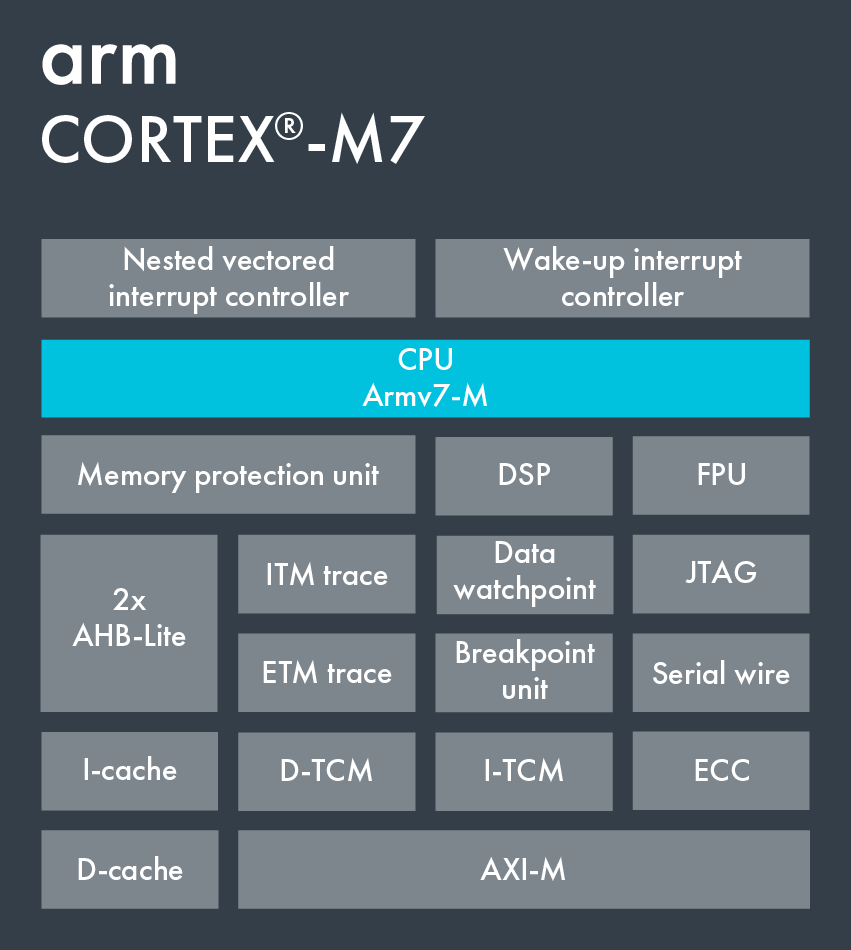
\includegraphics[width=.7\textwidth]{./Figures/Cortex-M7.png}
    \caption{Diagrama de la arquitectura \emph{Cortex M7}\protect\footnotemark.}
	\label{fig:cortexm}
\end{figure}

\footnotetext{Imagen tomada de la página oficial de \emph{ARM Developers}. \citep{WEBSITE:cortexm}}

La arquitectura tiene un módulo que permite programar y depurar el integrado.
Este módulo se denomina \emph{CoreSight} y es propio de los dispositivos \emph{ARM}.
En la figura \ref{fig:coresight} se muestra un diagrama en bloques del módulo.
Sus partes principales son:

\begin{itemize}
    \item \emph{Cross Triggering}: permite conectar y encaminar las señales que utilizan las sondas de depuración.
        En la figura \ref{fig:coresight} está representada en los bloques \emph{CTI}.
        Además, se unen a través del \emph{Cross Trigger Matrix (CTM)}.
    \item \emph{Debug Access Port (DAP)}: es el puerto físico para conectar la sonda de depuración. Es una implementación de la interfaz de depuración \emph{ARM}.
    \item \emph{Embedded Trace Macrocells}: permite extraer información y controlar el núcleo del dispositivo.
    \item \emph{Instrumentation Trace Units}: permite que una sonda de depuración se conecte con las \emph{Embedded Trace Macrocells}.
    \item \emph{ROM Tables}: sirven para que la sonda de depuración identifique al integrado.
    \item \emph{Self Hosted Debug}: son instrucciones específicas de depuración controladas por un procesador secundario.
    \item \emph{Trace Interconnect}: provee puentes para compartir señales de reloj, alimentación y otras señales comunes.
\end{itemize}

\begin{figure}[htbp]
	\centering
	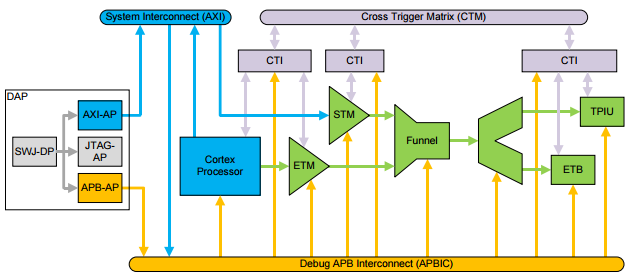
\includegraphics[width=\textwidth]{./Figures/coresight.png}
    \caption{Diagrama del módulo \emph{CoreSight}\protect\footnotemark.}
	\label{fig:coresight}
\end{figure}
\footnotetext{Imagen tomada del artículo \emph{How to debug: CoreSight basis}. \citep{WEBSITE:coresight}}

\section{Servidores y sondas de depuración}
\label{sec:depuracion}

Una sesión de depuración sirve para observar y modificar el estado de ejecución de un programa.
Esto se logra al leer y modificar los valores en registros del procesador y periféricos.
Además, se necesita de un sistema de disparos por eventos y supervisión de recursos.
Finalmente, la sesión debe detener la ejecución del núcleo de ser necesario.
En la figura \ref{fig:debug} se puede observar un esquema simplificado de una sesión de depuración.

\begin{figure}[htbp]
	\centering
	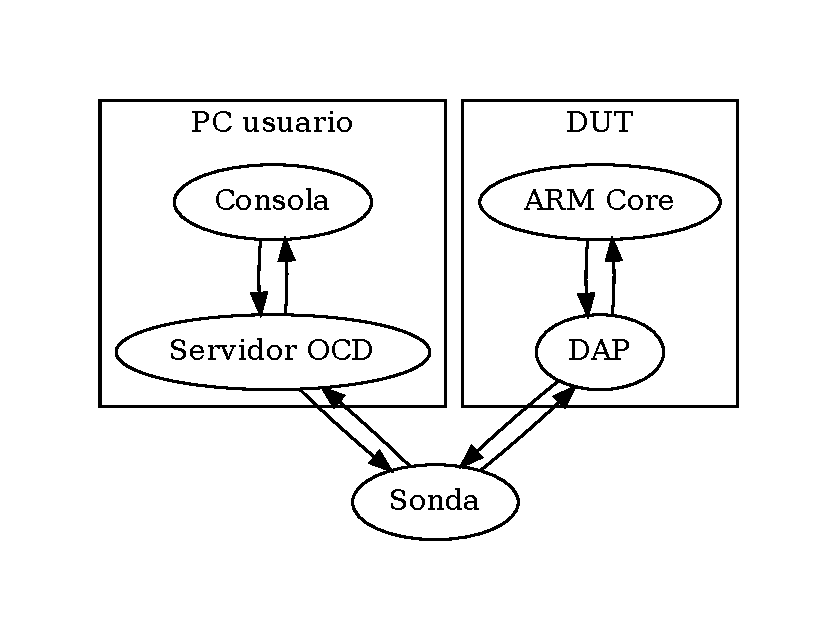
\includegraphics[width=.8\textwidth]{./Figures/debug.pdf}
    \caption{Conexión de una sesión de depuración.}
	\label{fig:debug}
\end{figure}

Un servidor \emph{On-chip debugger (OCD)} tiene la misión de abstraer la conexión de la sonda de depuración.
Además, facilita el manejo del ciclo de vida de la sesión y permite usar un \emph{software} como \emph{GNU Project debugger (GDB)}.
Finalmente, es la base de una pila de tecnologías que permite el uso de herramientas como \emph{GNU Emacs (Emacs)} \citep{BOOK:gdb}.
En la tabla \ref{tab:servidores} se puede observar un resumen de los servidores evaluados en el trabajo.

\begin{table}[h]
	\centering
	\caption[Servidores de depuración]{Comparativa entre servidores de depuración}
	\begin{tabular}{l c c c}    
		\toprule
        \textbf{Servidor} & \textbf{API} & \textbf{Acceso}   & \textbf{Licencia}\\
		\midrule
        OpenOCD           & tcl                         & Registros y SDRAM & MIT\\        	
        PyOCD             & Python 3                    & Registros y SDRAM & Apache-2.0\\
		\bottomrule
		\hline
	\end{tabular}
	\label{tab:servidores}
\end{table}

El servidor OCD utilizado en este trabajo es PyOCD.
La principal característica que lo diferencia es el uso de Python 3 como lenguaje de \emph{scripting}.
Además, provee un servidor GDB, permite la programación de memoria \emph{flash} y ofrece una interfaz por consola de comandos \citep{WEBSITE:pyocd}.
Finalmente, los datos mas relevantes son:

\begin{itemize}
    \item Requerimientos:
        \begin{itemize}
            \item Python 3.6.0 o superior.
            \item Una versión reciente de libusb.
            \item macOS, GNU Linux, Windows 7 o FreeBSD.
        \end{itemize}
    \item Sondas de depuración soportadas:
        \begin{itemize}
            \item Atmel EDBG/nEDBG.
            \item Atmel-ICE.
            \item Cypress KitProg3 o MiniProg4.
            \item DAPLink.
            \item Keil ULINKplus.
            \item NXP LPC-LinkII
            \item NXP MCU-Link
            \item PE Micro Cyclone y Multilink.
            \item Raspberry Pi Picoprobe.
            \item SEGGER J-Link.
            \item STLinkV2 y SRLinkV3.
        \end{itemize}
\end{itemize}




Las sondas de depuración tienen el objetivo de conectar el \emph{Debug Access Port} con el puerto del ordenador del usuario.
Adaptan los niveles de tensión y los protocolos involucrados.
Luego, permiten realizar una sesión de depuración, programar el dispositivo o verificar el estado de los componentes en la placa.
En la figura \ref{fig:sonda} se puede ver la sonda provista por el cliente.

\begin{figure}[htbp]
	\centering
	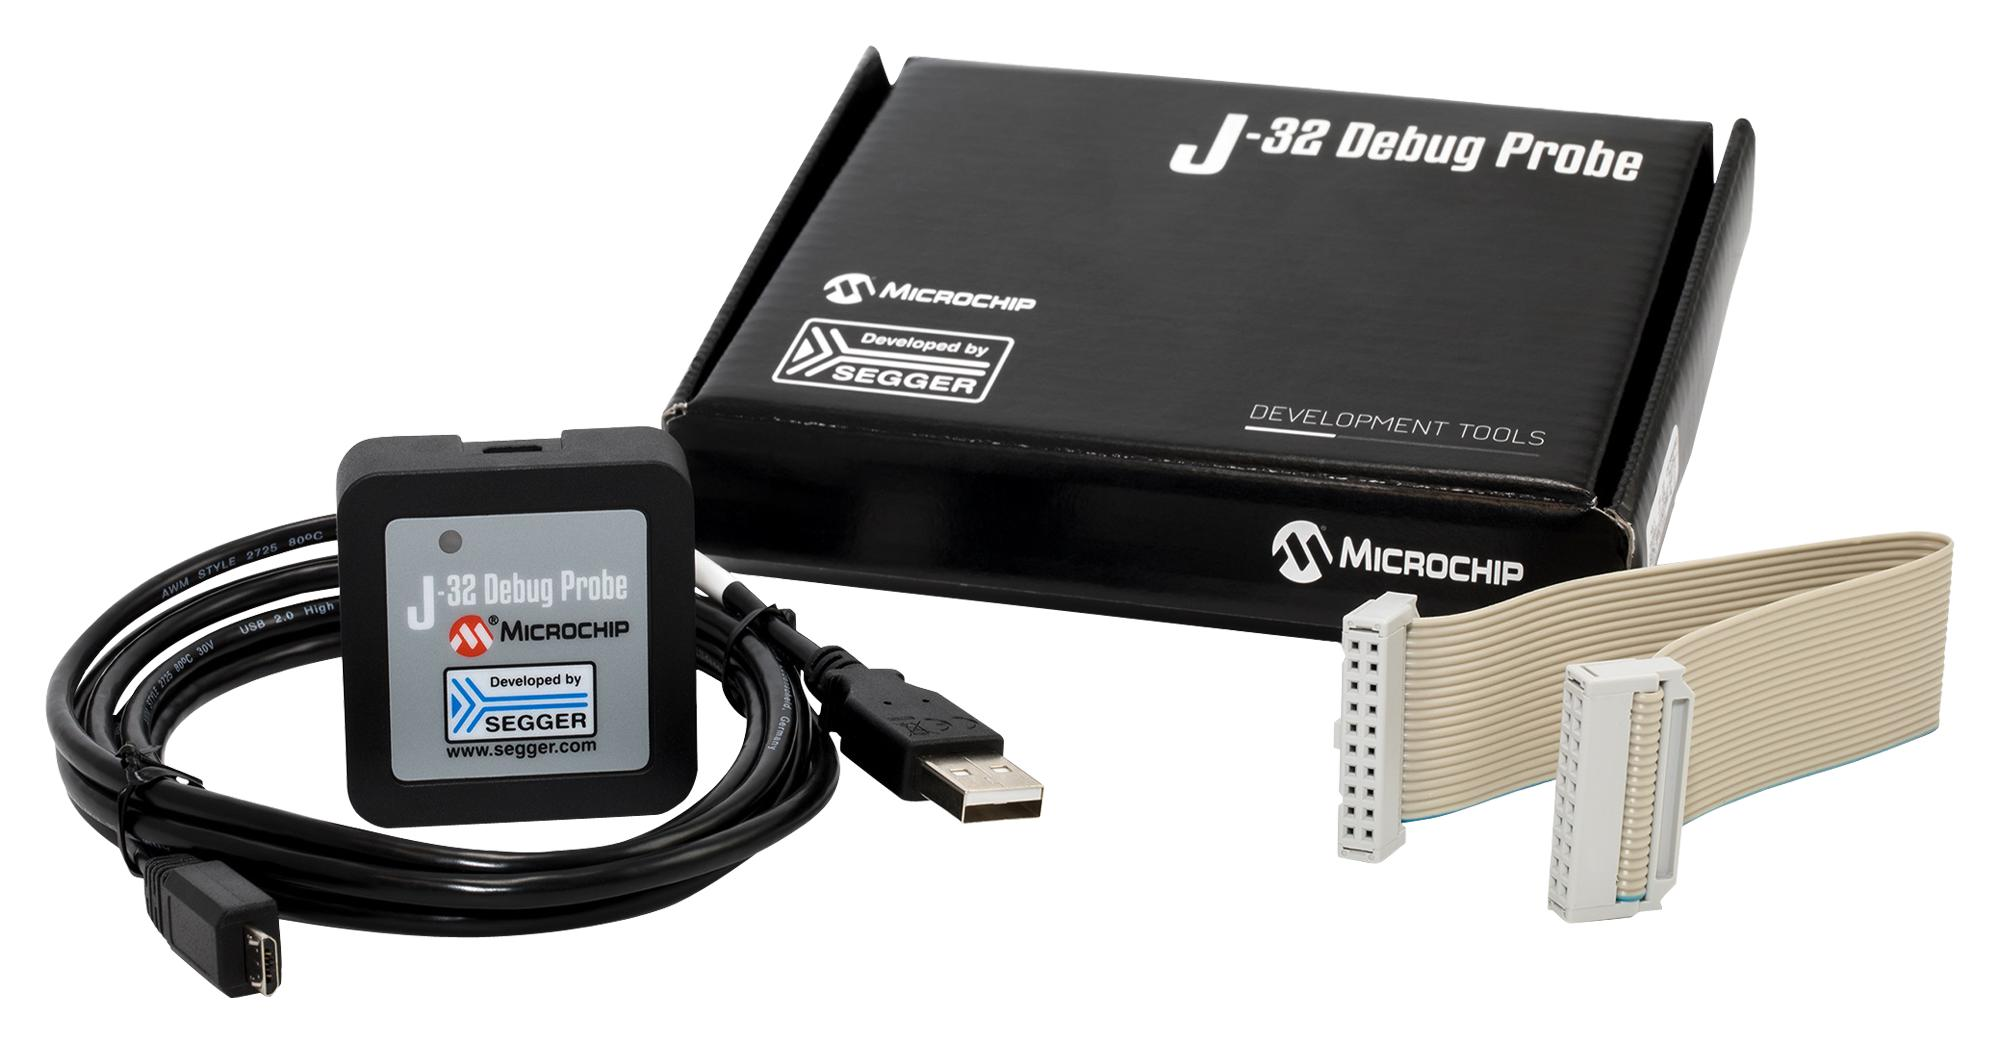
\includegraphics[width=.8\textwidth]{./Figures/segger.jpg}
    \caption{Sonda de depuración \emph{Segger J-32}\protect\footnotemark.}
	\label{fig:sonda}
\end{figure}
\footnotetext{Imagen tomada de \url{https://www.digikey.com/}}

\section{Periféricos de interés}
\label{sec:perifericos}

El dispositivo bajo prueba ofrece una variedad de periféricos para el desarrollo de aplicaciones.
Sin embargo, el cliente manifestó interés solo en los que se nombran a continuación:
\begin{itemize}
    \item CAN: este periférico permite al microcontrolador ser el dispositivo principal en una \emph{Controller Area Network}. La red es de grado industrial y fue diseñada para gestionar una red de sensores en un ambiente automotriz.
    \item PIO: es el puerto de entradas y salidas digitales de propósito general. En el caso del dispositivo bajo prueba, el periférico permite usar circuitos anti rebote, \emph{pull-up} y \emph{pull-down} internos. 
    \item SPI: el periférico permite realizar una conexión del tipo \emph{Serial Peripheral Interface}. Esta conexión es sincrónica y solo apta para distancias cortas.
    \item UART: es un periférico que permite conectarse a puertos y controlar dispositivos serie.
    \item Watchdog: el periférico sirve para detectar un error de ejecución y reiniciar el microprocesador.
\end{itemize}

En la tabla \ref{tab:perifericosresumen} se resume la funcionalidad de cada uno de ellos.

\begin{table}[h]
	\centering
	\caption[Resumen de periféricos]{Resumen de periféricos.}
	\begin{tabular}{l c c}    
		\toprule
        \textbf{Periférico} & \textbf{Funcionalidad}\\
		\midrule
		CAN                 & Bus de comunicación de grado industrial\\        	
		PIO                 & Entradas y salidas digitales\\
		SPI                 & Interfaz de comunicación sincrónica\\
		UART                & Puerto para dispositivos serie\\
		Watchdog            & Detección de errores y reinicio del integrado\\
		\bottomrule
		\hline
	\end{tabular}
	\label{tab:perifericosresumen}
\end{table}

\newpage

\section{Entornos de desarrollo}
\label{sec:entornos}

Para escribir el código que corre en el dispositivo bajo prueba se utilizó un entorno integrado de desarrollo (IDE).
Este IDE es MPLAB y fue provisto por el fabricante del integrado.
MPLAB está compuesto por una colección de programas que trabajan como un único sistema.
Entre ellos se encuentran:

\begin{itemize}
    \item Compilador para lenguaje C.
    \item Biblioteca CMSIS de ARM.
    \item Biblioteca HARMONY 3 de Microchip.
    \item Herramienta gráfica para la planificación de terminales.
    \item Herramienta gráfica para la configuración de periféricos.
    \item Herramienta gráfica para la configuración de reloj.
    \item Cliente GDB para sesiones de depuración.
\end{itemize}

Para realizar el código del inyector por consola de comandos se utilizó el lenguaje de programación Python 3.
Es un lenguaje interpretado que permite escribir código portable.
Además, el intérprete tiene la capacidad de crear ambientes virtuales.
Un ambiente virtual es un espacio de trabajo donde las dependencias instaladas quedan encapsuladas.
De esta manera, se puede simular el despliegue en un ambiente de producción.
Finalmente, junto al intérprete se utilizó un gestor de paquetes llamado PIP.
Esto facilitó la instalación automática del sistema.

Para escribir el código en Python 3, el \emph{firmware} en C y esta memoria en \LaTeX, se utilizó el editor de texto Neovim.
Este programa está basado en el editor Vi de los sistemas Unix.
Su funcionamiento es modal, esto significa que el editor funciona en los siguientes modos:

\begin{itemize}
    \item Modo normal:
        \begin{itemize}
            \item Navegar el documento.
            \item Ejecutar comandos de consola con la posibilidad de volcar el \emph{standard output} en el documento.
            \item Ejecutar \emph{scripts} de Neovim que permiten, por ejemplo, ordenar alfabéticamente una lista.
            \item Ejecutar búsquedas y reemplazos con comandos \emph{sed}.
            \item Grabar y ejecutar macros.
        \end{itemize}
    \item Modo inserción: permite escribir en el documento.
    \item Modo visual: permite seleccionar bloques del documento para aplicar comandos.
    \item Modo terminal: es un \emph{buffer} que emula una terminal Unix.
\end{itemize}

Neovim tiene la capacidad de conectarse a un servidor de análisis sintáctico de un lenguaje en particular.
Esto lo logra a través del \emph{Language Server Protocol (LSP)}.
El protocolo permite que un demonio realice el análisis de la sintaxis del código y envíe al editor información sobre errores y advertencias.
De esta manera se separa al editor del análisis sintáctico del lenguaje.
Además, Neovim tiene incorporado los diccionarios de la mayoría de los idiomas. Con solo ejecutar \texttt{:set spelllang=es} y \texttt{:set spell}, el editor resalta las palabras que no estén escritas en correcto castellano.

El último elemento del flujo de trabajo es el multiplexor de terminal Tmux.
Este programa permite dividir la terminal, crear \emph{buffers} y crear o conectarse a sesiones locales y remotas.
Esto posibilita partir una terminal y trabajar en simultáneo en dos o más ordenadores.
Finalmente, se trabajó de forma integrada con un ambiente de laboratorio remoto y sistemas de desarrollo locales.
En la figura \ref{fig:nvim} se puede ver un ejemplo del flujo de trabajo.

\begin{figure}[htbp]
	\centering
	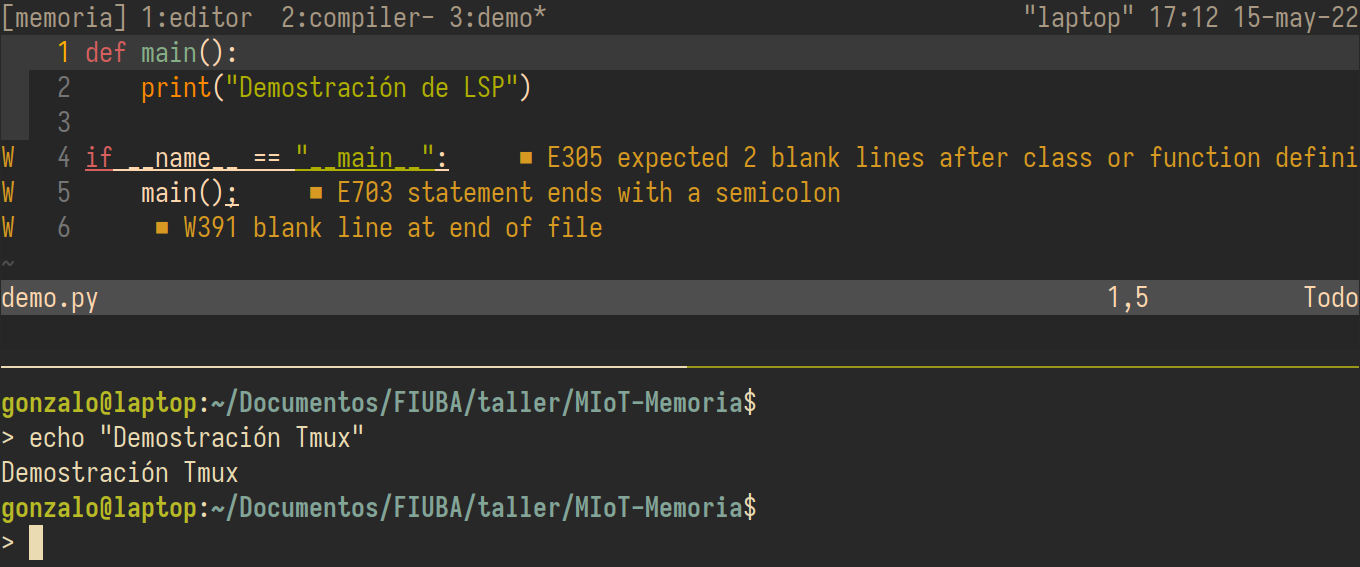
\includegraphics[width=\textwidth]{./Figures/nvimtmux.png}
    \caption{Ejemplo del flujo de trabajo Tmux-Neovim.}
	\label{fig:nvim}
\end{figure}

\newpage

\section{Requerimientos del cliente}
\label{sec:emphuerimientos}

Se realizaron una serie de reuniones con el cliente y se pudo definir los requerimientos del trabajo.
A continuación se enumeran los principales:

\begin{enumerate}
	\item Referentes al inyector por consola de comandos:
		\begin{enumerate}
			\item Generará de una interfaz de usuario.
			\item Permitirá configurar el ensayo a realizar.
			\item Observará la salida del dispositivo bajo prueba.
            \item Inyectará \emph{soft-errors} en el dispositivo bajo prueba.
			\item Persistirá las operaciones, entradas y salidas.
			\item Generará informes del ensayo realizado.
		\end{enumerate}
	\item Referentes al proceso del dispositivo bajo prueba:
		\begin{enumerate}
			\item Verificará el estado de los periféricos del dispositivo bajo prueba.
			\item Detectará si el dispositivo bajo prueba perdió su secuencia.
			\item Generará reportes de estado de periféricos y secuencia.
			\item Permitirá que el inyector por consola de comandos configure el alcance de la secuencia.
			\item Permitirá que el inyector por consola de comandos maneje el flujo de su secuencia.
		\end{enumerate}
\end{enumerate}

El cliente definió algunas restricciones para el desarrollo del sistema.
Estas se enumeran a continuación:

\begin{itemize}
	\item Utilización de un repositorio con control de versiones \emph{Gitlab}.
	\item Documentación del código con \emph{Doxygen}.
	\item Utilización exclusiva del lenguaje de programación \emph{Python 3}.
\end{itemize}

